%
% introduction.tex
%
% Copyright (C) 2019 by Universidade Federal de Santa Catarina.
%
% OBDH 2.0 Documentation
%
% This work is licensed under the Creative Commons Attribution-ShareAlike 4.0
% International License. To view a copy of this license,
% visit http://creativecommons.org/licenses/by-sa/4.0/.
%

%
% \brief Introduction chapter.
%
% \author Gabriel Mariano Marcelino <gabriel.mm8@gmail.com>
%
% \institution Universidade Federal de Santa Catarina (UFSC)
%
% \version 0.1.0
%
% \date 18/07/2019
%

\chapter{Introduction} \label{ch:introduction}

\begin{itemize}
    \item Main target: FloripaSat-2
    \item Improved version of the OBDH from FloripaSat-1
    \item Open source software (GPLv3 license)
    \item Open source hardware (GPLv3 license)
    \item RTOS
    \item Low power MCU
\end{itemize}

\begin{figure}[!ht]
    \begin{center}
        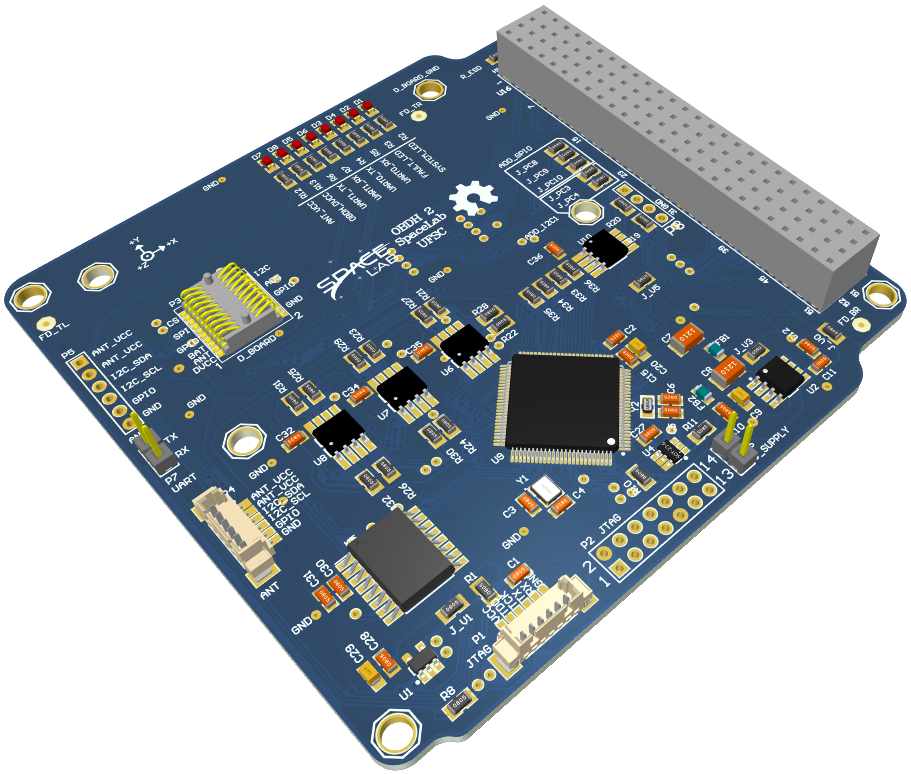
\includegraphics[width=0.75\textwidth]{figures/obdh2-pcb-3d.png}
        \caption{3D view of the OBDH 2.0 PCB.}
        \label{fig:pcb-3d}
    \end{center}
\end{figure}
